\documentclass[a4paper, 12pt]{article}
\usepackage[english, russian]{babel}
\usepackage[T2A]{fontenc}
\usepackage[utf8]{inputenc}
\usepackage{graphicx}
\usepackage{stmaryrd}
\usepackage{amsmath}
\usepackage{amssymb}
\usepackage{amsfonts}
\usepackage{array}
\usepackage{booktabs}
\usepackage{wrapfig}
\usepackage{caption} 
\usepackage{listings}
\usepackage{float} 

\begin{document}
    \begin{center}
        \subsubsection*{Отчёт по практическим заданиям}
        \subsubsection*{Прикладная математика. Лекция №2.}
    \end{center}

    \quad \textbf{Задача.} Провести изоляцию корней и найти их значения для заданых уравнений:
    \begin{center}
        1) $x - \sin(x) = 0.25$;
        2) $e^x - x^2 = 0$;
        3) $x^3  + 3x^2 - 24x + 1 = 0$;
    \end{center}

    \quad \textbf{Решение.} (/practical-tasks/nonlinear-equals/task-12.m) Для решения этих уравнений я использовал бинарный поиск (бисекцию), метод Ньютона-Рафсона и метод Секущих. Соотвествующие методы описаны в файлах в виде функций с соотвествующимим названиями, я лишь поясню специфику их реализации.

    \quad \textbf{RootSeparation} - функция для отделения корней заданой функции. Она принимает на вход саму функцию $f$, отрезок для поиска корней $\left[ a, b\right]$, интервал с которым ищутся корни $e$ и $PlotFlag$, отвечающий за построение графика функции и выделения промежутков с корнями. Все ниже приведённые графики это результат выполнения $RootSeparation$ c $PlotFlag = 1$.
    $e$ - очень важный параметр, т. к. для, например, сильно осцелирующих функций некоторые корни по ходу выполнения функции могут пропускаться. 

    \quad Для определения промежутка на котором встречаются корни, можно первоначально построить график функции и визуально определить в каких точках функция обращается в ноль. Возвращает функция два массива левых и правх границ промежутков, на которых точно есть корни. 

    \quad \textbf{edit\_bisection} - функция реализующая метод поиска корня функции $f$, на интервале $\left[a, b\right]$. Аналогично $RootSeparation$ есть параметр $PlotFlag$ для построения графика.
    
    \quad \textbf{newton\_method} - реализация метода Ньютона-Рафсона, параметры аналогично.

    \quad \textbf{secant\_method} - реализация метода секущих (модификация метода Ньютона-Рафсона), параметры аналогично. 

    \newpage

    1) Рассмотрим уравнение $x - \sin{x} = 0.25$. Визуально корень точно есть на промежутке $\left[ 0, 2 \right]$. Результат трёх методов $x = 1.1713$.

    \begin{figure}[H]
        \centering
        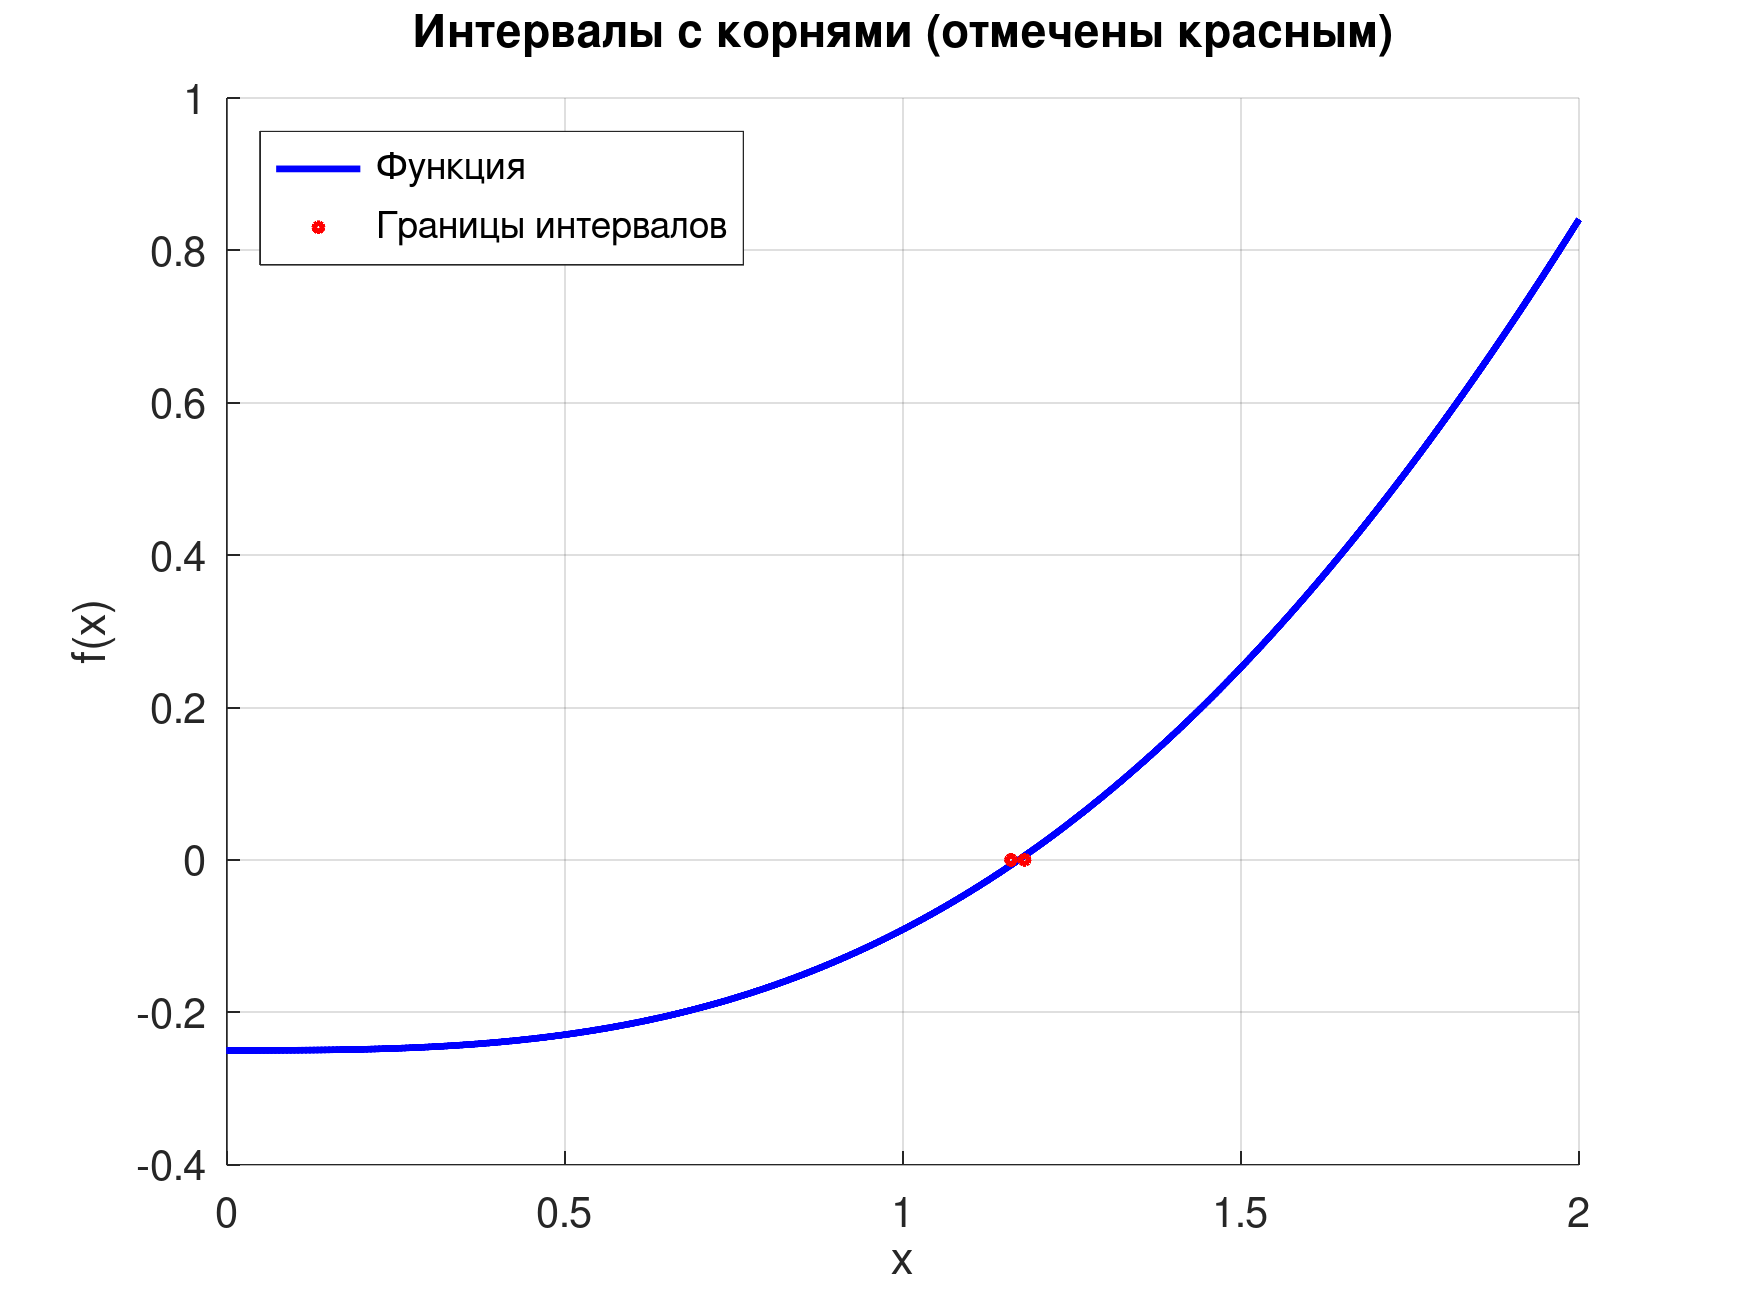
\includegraphics[width=0.7\textwidth]{../reports/.png/xsinx.png}
        \caption{Визуализация $x - \sin{x} = 0.25$}
    \end{figure}

    2) Рассмотрим уравнение $e^x - x^2 = 0$. Визуально корень точно есть на промежутке $\left[-1, 0\right]$. Результат трёх методов $x = -0.7025$.

    \begin{figure}[H]
        \centering
        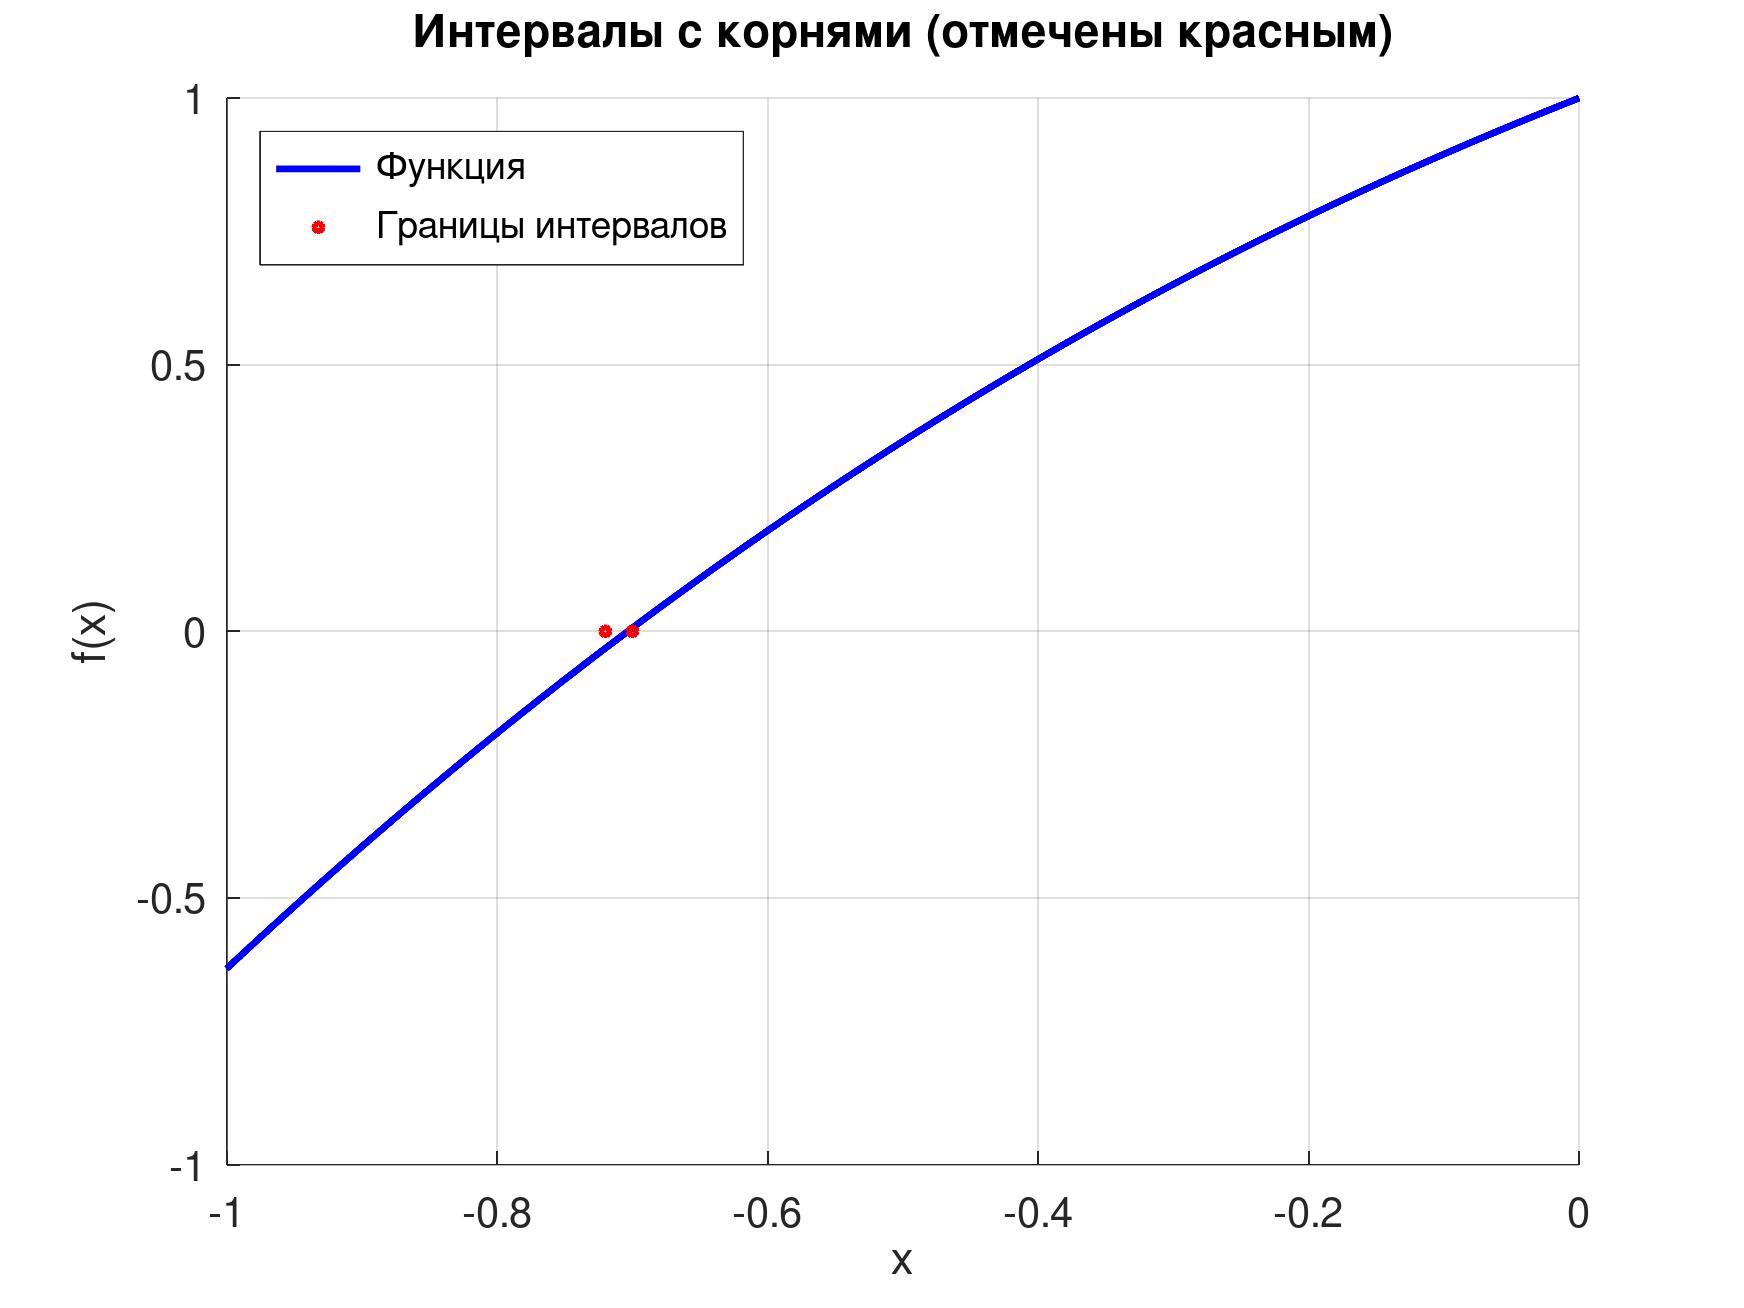
\includegraphics[width=0.7\textwidth]{../reports/.png/exx2.png}
        \caption{Визуализация $e^x - x^2 = 0$}
    \end{figure}

    3) Рассмотрим уравнение $x^3 + 3x^2 - 24x + 1 = 0$. Визуально корень точно есть на промежутке $\left[-8, 6\right]$. Результат трёх методов: 
    
    \centering $\forall x \in \left\{ -6.637500, 0.042500, 3.596250 \right\}$.

    \begin{figure}[H]
        \centering
        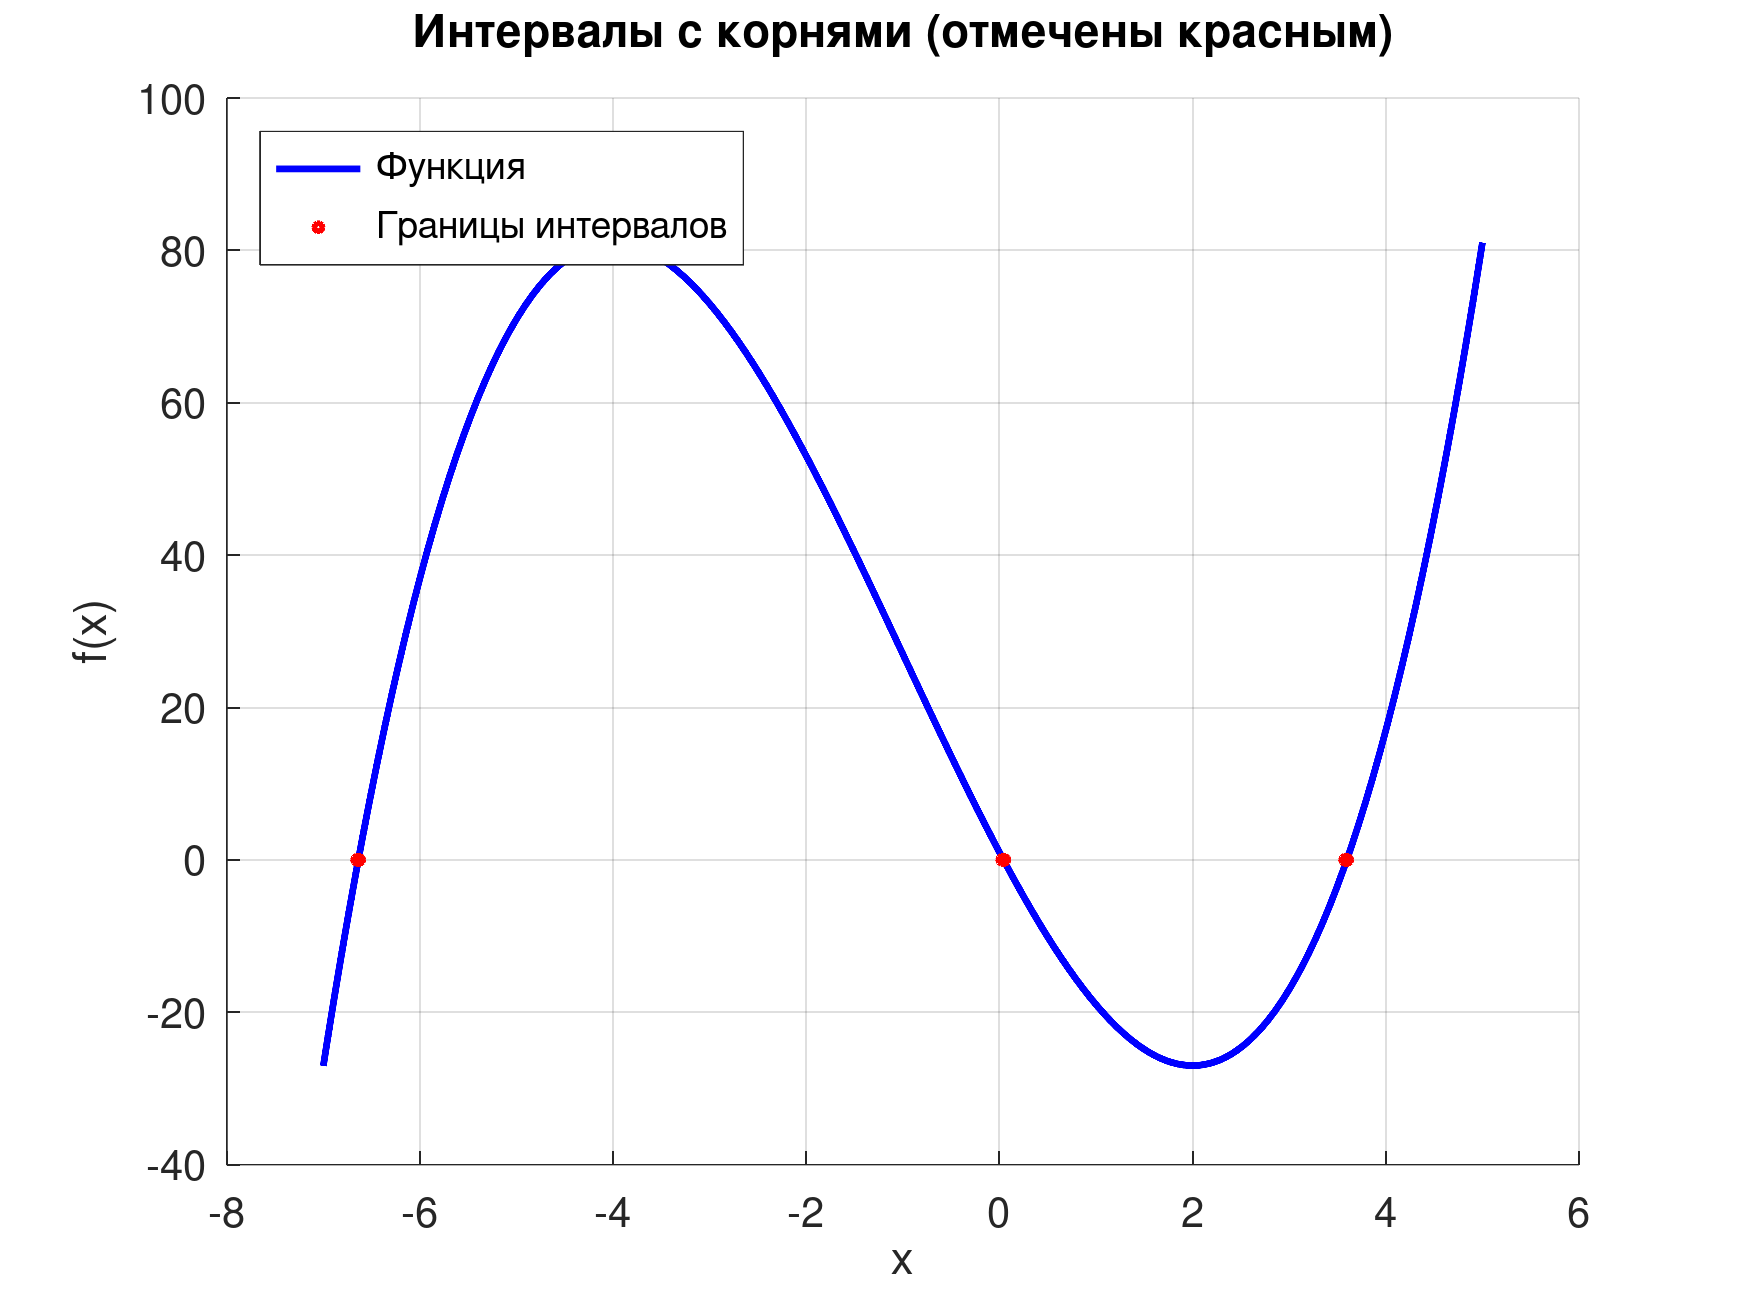
\includegraphics[width=0.7\textwidth]{../reports/.png/x3.png}
        \caption{Визуализация $x^3 + 3x^2 - 24x + 1 = 0$}
    \end{figure}

    \end{document}
\end{document}